\documentclass[10pt,a4paper,oneside]{article}
\usepackage[swedish]{babel}
\usepackage[utf8]{inputenc}
\usepackage[T1]{fontenc}
\usepackage{amsmath}
\usepackage{amsfonts}
\usepackage{graphicx}
\usepackage{hyperref}
\usepackage{url}
\usepackage[nomarkers]{endfloat}
\renewcommand{\efloatseparator}{\mbox{}} 
\mdseries\itshape\urlstyle{same}

\usepackage{titling}
\predate{\begin{center}\placetitlepicture\large}
\postdate{\par\end{center}}
 
 \newcommand{\titlepicture}[2][]{%
  \renewcommand\placetitlepicture{%
    \includegraphics[#1]{#2}\par\medskip
  }%
}
\newcommand{\placetitlepicture}{}


\begin{document}

\title{Vågkraft \\ 
\large }
\author{\small Johanna Sörbom}
\date{\small \today}
\titlepicture[width=3in]{Wave}

\maketitle
\newpage

\section{Sammanfattning}
Vågkraft är en relativt ny energiteknik med stor potential. Världens totala potentiella vågenergi kan uppskattas till 2 TW, vilket är av ungefär samma ordning som världens totala elanvändning. Men idag används endast en bråkdel av denna energi. Att vågkraften inte är mer utbredd idag beror på barriärer i form av teknik, ekonomi, planering och licenser samt infrastruktur. Vågkraftteknik är betydligt dyrare än andra former av förnybar energi och detta måste förändras för att ge vågkaften en chans att växa. För att detta ska ske krävs fortsatt forskning och investeringar. I denna uppsats kommer dessa barriärer att presenteras och disskuteras för att besvara frågan om varför vågkraften inte är mer utbredd.  \newpage

\tableofcontents
\newpage

\section{Inledning}
Vindkraft är en energiform som har användas i många olika former under under människans historia \cite{Elliott}. Så tidigt som 5000 år före kristus utnyttjades vindens kraft för att driva båtar längs med Nilen och väderkvarnar användes för pumpa vatten i Kina. Sedan dess har nya sätt att utnyttja vindens energi utvecklats och spridits runt om i världen \cite{WEF}. Vågkraft är ett relativt nytt sätt att utnyttja vindens energi. När vind rör sig över vatten skapas vågor genom friktionskraft som lagrar vindens energi under en tidsperiod \cite{Elliott}. Om all denna energi utvanns så skulle det räcka för att täcka hela jordens elkonsumtion \cite{Cruz}. Så varför gör den inte redan det? Denna rapport kommer att presentera vågkraftens potential samt analysera de problem som står i vägen för en storskalig utvinning av vågkraft i världen. 

\section{Metod}
Denna uppsats har begränsat sig till inte gå altför djupgående in på de tekniska aspekterna av vågkraft och ämnar endast till att skapa en överblick över den problematik som vågkraften står inför. Uppsatsen hålls objektiv och inga personliga åsikter presenteras. 

Denna uppsats grundar sig på främst på rapporter och utvärderringar av vågkraft som energiresurs. Den källa som har användts mest är en Wave energy technology brief från IRENA. Detta är en mallanstatlig organisation som stödjer länder i deras övergån till förnybar energi. Utgivningsåren varierar från källa till källa men är till störst del relativt nya.

Viktigt att tänka på är att källorna kan vara vinklade och författaren kan tänkas uttrycka sina egna åsikter. Källan IRENA som använts till stor del i denna rapport kan t.ex tänkas ha en mycket possitiv syn på vågkraft. Denna uppsats har försökt hålla en så objektiv synvinkel som möjligt.  Med något undantag endast vetenskapliga rapporter från olika författare användts i denna uppsats för att göra denna uppsats så tillförlitlig och objektiv som möjligt. En artikel från YaleEnviromental 360 har använts som källa i denna uppsats. Informationen från denna källa har bedömts pålitlig nog att ha med i uppsatsen.\newpage



\section{Vågkraft idag}
Vågenergi är en biprodukt av atmosfärens omdistrubering av solenergi som uppstår när vind rör sig över vatten \cite{Cruz}. Vågkraft kan däför indirekt ses som en typ av både vind- och solkraft. Men till skillnad från vindkraft så rör sig vatten i föränderliga cirkulära mönster som gör att teknik för utvinning av vågkraft är mycket olik den för vindkraft \cite{Elliott}. Det finns idag en mängd olika tekniker för att utvinna vågkraft. Se figur \ref{Technologies} för en sammanfattning av dagens vågkrafttekniker \cite{IRENA}.

Sedan 1970-talet har vågkraftstekniken sett en stor utveckling och de system som fungerar bäst är idag bland annat Pelamis wave snake, Oysters ostronliknande oscilerande flärpar och Wavegens strandmonterade  OWCs \cite{Elliott}. På den Svenska marknaden finns Fortum som tillsammans med Seabased år 2016 kopplade in den första vågkraftsparken om 1MW till det nordiska elnätet. Dessa vågkraftverk består av bojar kopplade till linjärgeneratorer som utnyttjar höjdskillnaden mellan vågtopp och vågdal för att utvinna energi \cite{Fortum}. Det finns även fungerande vågkraftparker eller projekt i bland annat Storbritannien \cite{Yale}.  


\section{Vågkraftens potential}
Världens totala potentiella vågenergi kan uppskattas till 2 TW, vilket är av ungefär samma ordning som världens totala elanvändning. Av detta är det rimligt att anta att bara 10-25 procent av denna energi kan utnytjas. Detta betyder att vi inte endast kan förlita oss på vågkraft, men det skulle potentiellt kuna bidra med en stor mängd av den energi som vi människor använder. Vågkraftens främsta fördelar är att den kommer i en högkvalitativ form av mekanisk svängningoscillation och att den färdas långa avstånd med liten förlust. Mängden energi som överförst till vågor är vanligtvis mellan \begin{math} 0.01  \end{math} till \begin{math} 0.1 W/m^2 \end{math} men byggs upp under de långa sträckor som vågorna färdas och landar i snitt på 100 kW/m. Den genomsnittliga årliga mängd energi som kan utvinnas globalt genom vågkraft representeras grafiskt i figur \ref{Globalmean} \citep{Cruz}. 

\section{Drivkrafter och barriärer}
Vågkraftens potential driver på utvecklingen av vågkraft på många ställen världen över. Den har liten miljöpåverkan och liten synlighet på kuststräckor. Detta har lett till stöd från regeringar och och den privata sektorn och fler och fler kommersiella vågkraftprojekt och testplaster annonseras. Men utvecklingen av en optimal vågkraftteknik är långt ifrån klar och haven utgör en hård miljö för tekniken att frodas. Förutom de tekniska utmaningarna så möter vågkraft liknande problem som havsbaserade vindkraft gör. Dessa är: osäker miljöpåverkan, investeringskrav, otillräcklig infrastruktur samt planering och licens procedurer \cite{IRENA}. Vid utveckling och implementering av vågkraft är det viktigt att komma ihåg att vågkraft inte bara handlar om tekniken. Enligt Summerton bör man inte dra en skart linje mellan tekniken och samhället. Alla stora tekniska system bör ses som sociotekniska system och ta hänsyn till icke tekniska aspekter. Detta kommer att disskuteras vidare i avsittet Planering och Liicencer där vågkraftens samhällets inställning till tekniken visas spela stor roll i hur lyckad implementeringen av denna blir.  HÅRD

\subsection{Teknik}
Ett av de centrala problemen är komplexiteten vid utvinning av vågkraft. Det finns idag en mängd olika tekniker för att utvinna vågkraft men det finns tre huvudkategorier:  ocsilerande vattenkolumner som använder sig av en luftficka fångad i encylinder för att driva en turbin, ocsilerande kroppar som kan vara placerade både på havsbotten, på ytan eller i havet och använder vattnets rörelse för att utvinna energi samt "overtoping" omvandlare som använder en reservoar för att skapa fallhöjd och därigenom driva turbiner.

Vågkraft är även en svår teknologi att använda sig av när det kommer till miljön tekniken måste tåla att vistas i. Saltvatten är en oförlåtlig miljö som sliter mycket på tekniken och vågorna själva som rör sig åt alla möjliga håll gör det svårt att utveckla optimal teknik. Det räcker inte att ta hänsyn till vågornas höjd utan de har även en period som spelar in vid utvinning av energi \cite{Yale}.


\subsection{Miljöpåverkan}
Tidigare forskning från Uppsala universitet har visat att djur och natur inte verkar skadas av dessa kraftverk. Tvärtom skapar vågkraftverket artificiella rev där djur som krabbor kan leva \cite{Vattenfall}. Den huvudsakliga bieffekten av vågkraftinstalationer är minskning av vågor och höjd på vågorna som når kusten. Samtidigt är det viktigt att komma ihåg att vågkraft är en ung teknik och att det är svårt att veta vilken påverkan den kommer att ha på miljön på lång sikt. För att få bättre förståelse för den inverkan vågkraft kan ha på miljön har EU gått in och sponsrat ett project som har levererat ett antal guidelinjer för utvärdering av miljöpåverkan från vågkraftverk \cite{IRENA}. 

\subsection{Ekonomi}
De ekonomiska aspekterna vågkraft är, precis som vid utveckling av alla energikällor, av stor betydelse. Jämförelsevis är det betydligt dyrare att bygga havsbaserade vindkraftverk än att bygga de som placeras på land \cite{Yale}. 
Kostnaderna för vågenergiparker på 10MW uppskattas till mellan 330-630 EUR/MWh. Detta är betydligt högre än för andra typer av förnybar energi. Av denna kostnad uppskattas 22 procent gå till PTO systemet, 18 procent installation, 17 procent underhåll, och 5 procent uppkoppling till elnätet \cite{IRENA}.

Idag domineras vågkraften av start-ups och universitet som lever på lever på statligt stöd. För att göra vågkraften störres krävs en ny typ av investeringar. Utöver forskning, statliga stöd och stöd med policys så kommer det att krävas investeringar från privata företag \cite{IRENA}. Enligt Dave Levitan så kommer det troligtvis att krävas att större företag går in och investerar i utvecklingen för att den ska ta fart på samma sätt som utvecklingen av vindkraft. Men då dessa företag troligtvis väntar på att en optimal teknik ska framträda innan de investerar hamnar vågkrafttekniken i en ond cirkel där utvecklingen stannar av \cite{Yale}.Vågenergi skulle även kunna ses som ett sätt att bygga upp den havsrelaterade ekonomin och skapa en ny tillverkningsbas för energisystem i hav. Detta skulle kunna hjälpa varvsindustrin och fiskesamhällen att ta nytta av utvecklingen av vågkraft. T.ex så skulle fiskare även kunna få jobba med underhållning av vågkraftparkerna \cite{IRENA}. 

\subsection{Infrastruktur}
För att vågenergin ska få kunna förutsätta utvecklis krävs lämplig elnätinfrastruktur och tillgång till hamnar och hamn lokaler. Ett sätt att lösa detta problem är utvecklingen av “integrated offshore grid infrastructures”. Detta är något som utvecklas för havsbaserade vindkraft \cite{IRENA}. Genom att införa project med både vind och vågkraft skulle kostnaderna för detta kunna minskas och teknikerna skulle kunna komplementera varandra då de vågkraft kan producera el då vindkraftverken står still \cite{Yale}. Hamnar och hamn lokaler är också viktigt för storskaliga vågkraftprojekt. Att utföra underhåll av vågkraftparker är dyrt och de svåra havsförhållanderna gör det ännu dyrare. Att koppla bort vågkraftsomvandlarna och utföra underhållet på en säkrare och mer lättillgänglig plats i hamnen är ett alternativt tillvägagångssätt \cite{IRENA}. 

\subsection{Planering och licenser}
På grund av att vågkraft är stort beroende av geografiska förhållanden så skulle en förbestämd placeringsplan hjälpa sektorn att anpassa sig och överkomma sina lokala hinder. Kustsamhällen och utövare av traditionella havsbaserade aktiviteter kan ibland vara osäkra på vågkraftens inverkan på deras tillvaro. Det är därför viktigt att deras åsikter tas med i planeringen av vågkraften. Bristen på en planeringsprocess i områden men många olika intressen såsom transport, energi, fiske och turism tenderar att öka osäkerheten och riskerar förseningar för projekten \cite{IRENA}. 


\section{Avslutande diskussion och slutsats}
Vågkraft är en energiresurs som har stor potential. Men i nuläget finns det en hel del problematik som måste lösas innan vågkraften kan få en lika stor roll som vindkraften har i dagens samälle. 
Det är viktigt att komma ihåg att vågkraften är en relativt ny energteknik och att en jämförelse med vindkraft inte är rättvis om man inte tar hänsyn vindkraftens betydligt längre utvecklingperiod. Vågkraftteknik är betydligt dyrare än andra former av förnybar energi och detta måste förändras för att ge vågkaften en chans att växa. För att vågkraften ska kunna växa sig större krävs investering från större privata företag och inte endast små statliga bidrag. Kostnadsanalyser för att sänka kostnaderna samt utveckling innom infrastrukturen och tekniken för att kunna effektivisera vågkraften är också viktigt för att den ska kunna växa kommersiellt. Miljömässigt kommer forskning och kontinuelig analys av vågkraftens påverkan på djur och natur att krävas. Socialt är det även viktigt att utveckla sammarbeten med påverkade parter och ta vara på deras åsikter så att vågkraften kan gynna flera delar i samhället. Det kommer helt enkelt att krävas en hel del utveckling för att vågkraften ska kunna växa sig större. Det finns delade åsikter när det kommer kring hurvida vågkraften kommer att kunna bli en stadig källa till energi i vårat samhälle. Ett återkommande tema hos vågkraftexperter är att vågkraft är där vindkraft var för tre årtionden sedan. Trots alla dessa barriärer finns det hopp för vågkraften. Jason Busch från Oregon Wave Energy Trust säger att vi på 10 år har gått från att inte ha någon vågenergiteknik alls till att ha flera stycken project i haven som är nära att fungera för komerciellt bruk \cite{IRENA}. Hurvida vågkraften kommer att få större genomslag återstår att se. 
\newpage

\bibliographystyle{amsplain}
\bibliography{Wave}

\begin{figure}
\label{Globalmean}
	\includegraphics[scale=0.6]{globalmean.png}
	\caption{\r{A}rlig genomsnittlig v\r{a}gkraft [kW/m]}
\end{figure}

\begin{figure}
\label{Technologies}
	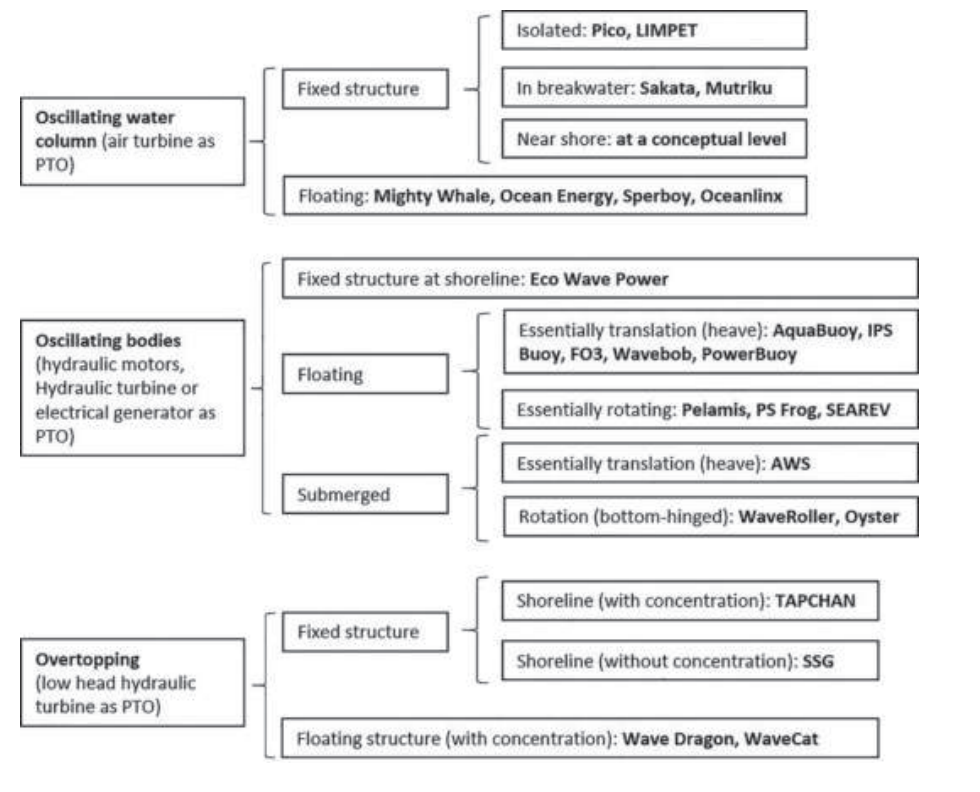
\includegraphics[scale=0.6]{Technologies.png}
	\caption{Wave energy technology}
\end{figure}


\end{document}